\documentclass[border=3mm]{standalone}

\usepackage{pgfplots}
\pgfplotsset{height=6cm,width=13cm,compat=1.15}

\begin{document}

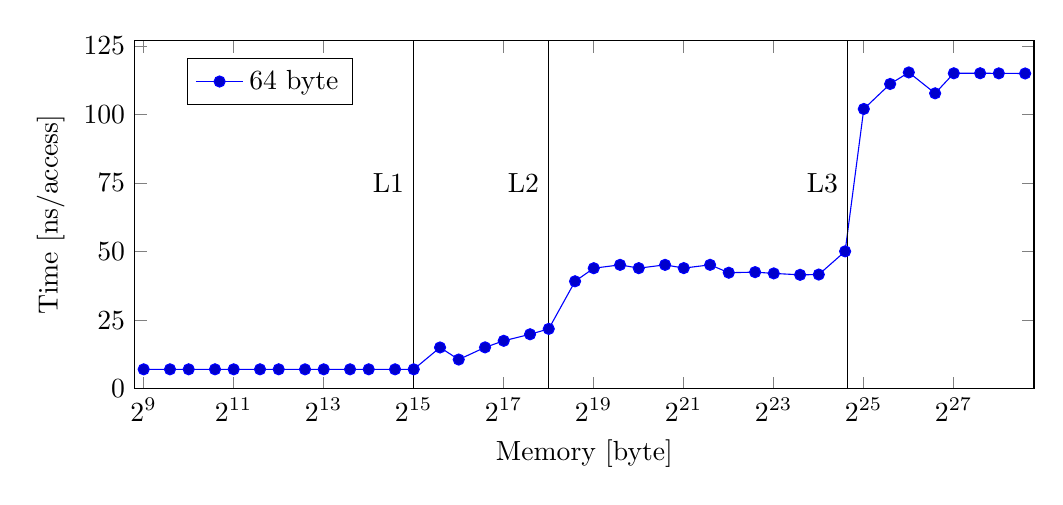
\begin{tikzpicture}
\begin{axis}[
	xmode=log,
	log basis x={2},
	ylabel={Time [ns/access]},
	xlabel={Memory [byte]},
	%scaled ticks=false,
	y tick label style={/pgf/number format/fixed},
	x tick label style={/pgf/number format/fixed},
	ytick distance={25},
	ymin = 0,
	%xmin = 64,
	enlarge x limits=0.01,
	legend style={at={(0.15, 0.95)}, anchor=north,legend columns=1},
	%ybar,
	% xtick=data,
	% bar width=7pt,
]
\addplot table {
512     7.069410165     134217728
768     7.070292546     134217728
1024    7.075352550     134217728
1536    7.071771845     134217728
2048    7.073846849     134217728
3072    7.072550951     134217728
4096    7.078295589     134217728
6144    7.062471986     134217728
8192    7.073067652     134217728
12288   7.072947769     134217728
16384   7.075867677     134217728
24576   7.063850782     134217728
32768   7.072181733     134217728
49152   15.037310466    134217728
65536   10.632586988    134217728
98304   15.072799800    134217728
131072  17.466243458    134217728
196608  19.845130615    134217728
262144  21.804437176    134217728
393216  39.159563273    134217728
524288  43.931234917    134217728
786432  45.146736766    134217728
1048576 43.948071286    134217728
1572864 45.146864067    134217728
2097152 43.970914895    134217728
3145728 45.156163694    134217728
4194304 42.286163175    134217728
6291456 42.497003108    134217728
8388608 42.032320461    134217728
12582912        41.514443442    134217728
16777216        41.618099474    134217728
25165824        50.073590972    134217728
33554432        101.978585253   134217728
50331648        111.089696241   134217728
67108864        115.294562050   134217728
100663296       107.675860745   134217728
134217728       114.982406912   134217728
201326592       115.003099651   134217728
268435456       114.958611745   134217728
402653184       114.912766150   134217728

};
%\addplot coordinates {(O0,0.034254) (O1,0.062424) (O2,4.4731) (O3,4.4157)};
\draw (32768,0) -- node[left]{L1} (32768, 150);
\draw (262144,0) -- node[left]{L2} (262144, 150);
\draw (26214400,0) -- node[left]{L3} (26214400, 150);


%\node[above] at (axis cs:O0,0.03177) {$\sim$0.03};
%\node[above] at (axis cs:O1,0.060008) {$\sim$0.06};

\legend{64 byte}
\end{axis}
\end{tikzpicture}

\end{document}
